\section*{Med hjælpemidler}
\begin{opgavetekst}{Opgave 1}
	\begin{center}
		\includegraphics[width=0.6\textwidth]{Billeder/chips}
	\end{center}
	Vægten af en pose chips (i gram) er approksimativt normalfordelt med den normalfordelte 
	stokastiske variabel
	\begin{align*}
		X \sim \textnormal{N}(120,2).
	\end{align*}
\end{opgavetekst}
\begin{delopgave}{}{1}
	Afgør, om en pose på 113 gram er et exceptionelt udfald.
\end{delopgave}
\begin{delopgave}{}{2}
	Forklar, hvad integralet 
	\begin{align*}
		\int_{120}^{123}\frac{1}{\sqrt{2\pi}2}e^{-\frac{1}{2}\left(\frac{x-120}{2}\right)^2}dx
		\approx 0.433
	\end{align*}
	siger om chipsposerne.
\end{delopgave}


\begin{opgavetekst}{Opgave 2}
	Fordelingsfunktionerne $F_X$ og $F_Y$ for to stokastiske variable
	\begin{align*}
		&X \sim \textnormal{N}(\mu_X,2)\\
		&Y \sim \textnormal{N}(\mu_Y,3)
	\end{align*}
	er givet på Figur \ref{fig:fordeling}.
	\begin{figure}[H]
		\centering
		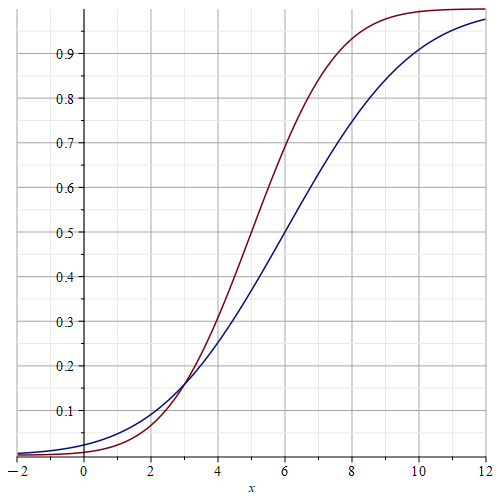
\includegraphics[width=0.6\textwidth]{Billeder/fordelinger}
		\caption{Graferne for fordelingsfunktionerne for $X$ og $Y$}
		\label{fig:fordeling}
	\end{figure}
	\phantom{h}
\end{opgavetekst}
\begin{delopgave}{}{1}
	Afgør hvilken af graferne der tilsvarer $F_X$ og hvilken, der tilsvarer $F_Y$.
\end{delopgave}
\begin{delopgave}{}{2}
	Bestem $\mu_X$ og $\mu_Y$.
\end{delopgave}
\begin{delopgave}{}{3}
	Bestem sandsynligheden $P(4<Y<8)$.
\end{delopgave}


\begin{opgavetekst}{Opgave 3}
	\begin{center}
		\includegraphics[width=0.6\textwidth]{Billeder/helpizza}
	\end{center}
	Hos en producent af pizzaer har man lavet en stikprøve på 100 pizzaer. Man har målt deres
	diameter, og antager at denne er normalfordelt. Resultatet af stikprøven kan findes 
	\href{https://github.com/ChristianJLex/TeachingNotes/raw/master/2023-2024/Data og lign/Pizzaradius.xlsx}{\color{blue!60} her.}
\end{opgavetekst}
\begin{delopgave}{}{1}
	Argumentér for at pizzaernes diameter er tilnærmelsesvist normalfordelte, og bestem den 
	estimerede middelværdi og estimerede spredning for den normalfordelte stokastiske variabel
	$X$, der beskriver diameteren.
\end{delopgave}
\begin{delopgave}{}{2}
	Bestem intervallet for de normale udfald for diameteren af pizzaerne.
\end{delopgave}
\begin{delopgave}{}{3}
	Bestem $z$-værdien for udfaldet 33cm og brug denne til at afgøre, om 33 er et exceptionelt
	udfald.
\end{delopgave}
\begin{meretekst}
	Producenten af pizzaer har en forventning om, at under 1$\%$ af deres pizzaer har en radius 	på under 29cm.
\end{meretekst}
\begin{delopgave}{}{4}
	Brug $X$ til at afgøre, om producenten opfylder sit ønske.
\end{delopgave}
\begin{meretekst}
	Producenten kan ikke ændre på spredningen af deres pizzaers diameter; de kan kun ændre på 
	middelværdien ved at tilføje lidt mere eller lidt mindre dej til hver pizza.
\end{meretekst}
\begin{delopgave}{}{5}
	\textbf{Ekstraopgave:} Bestem hvad middelværdien for $X$ skal være, hvis producenten skal
	opfylde sit ønske om, at kun 1$\%$ af pizzaerne har en diameter på under 29cm.
\end{delopgave}
